\begin{figure}[H]
  \centering
  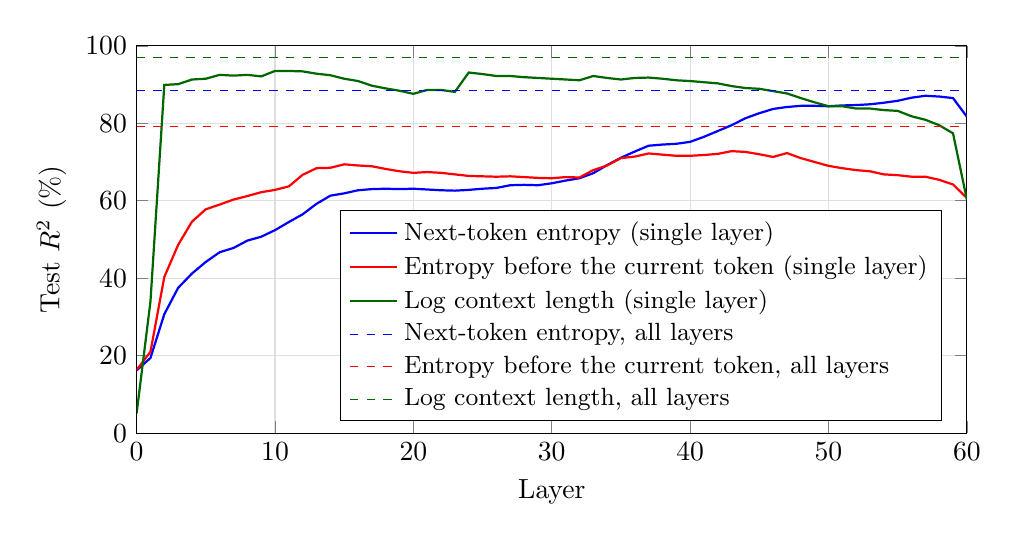
\begin{tikzpicture}
    \begin{axis}[
        width=\linewidth, height=6.5cm,
        xlabel={Layer}, ylabel={Test $R^2$ (\%)},
        xmin=0, xmax=60, ymin=0, ymax=100,
        xtick={0,10,20,30,40,50,60},
        grid=major, grid style={gray!25},
        legend pos=south east, legend cell align=left,
        legend style={font=\small},
      ]
      \addplot[thick, blue, mark=none] coordinates {
        (0,16.2) (1,19.4) (2,30.7) (3,37.5) (4,41.2) (5,44.2) (6,46.7) (7,47.8) (8,49.7) (9,50.7)
        (10,52.4) (11,54.5) (12,56.5) (13,59.2) (14,61.3) (15,61.9) (16,62.7) (17,63.0) (18,63.1) (19,63.0)
        (20,63.1) (21,62.9) (22,62.7) (23,62.6) (24,62.8) (25,63.1) (26,63.3) (27,64.0) (28,64.1) (29,64.0)
        (30,64.5) (31,65.2) (32,65.8) (33,67.1) (34,69.2) (35,71.1) (36,72.7) (37,74.2) (38,74.5) (39,74.7)
        (40,75.2) (41,76.5) (42,78.0) (43,79.5) (44,81.3) (45,82.6) (46,83.7) (47,84.2) (48,84.5) (49,84.5)
        (50,84.4) (51,84.6) (52,84.7) (53,84.9) (54,85.3) (55,85.8) (56,86.6) (57,87.1) (58,86.9) (59,86.5)
        (60,81.7)
      };
      \addlegendentry{Next-token entropy (single layer)}
      \addplot[thick, red, mark=none] coordinates {
        (0,16.3) (1,21.0) (2,40.3) (3,48.6) (4,54.6) (5,57.8) (6,59.0) (7,60.3) (8,61.2) (9,62.2)
        (10,62.8) (11,63.7) (12,66.7) (13,68.4) (14,68.5) (15,69.4) (16,69.1) (17,68.9) (18,68.2) (19,67.6)
        (20,67.2) (21,67.4) (22,67.2) (23,66.8) (24,66.4) (25,66.3) (26,66.2) (27,66.3) (28,66.1) (29,65.9)
        (30,65.8) (31,66.1) (32,66.0) (33,67.9) (34,69.1) (35,71.0) (36,71.4) (37,72.2) (38,71.9) (39,71.6)
        (40,71.6) (41,71.8) (42,72.1) (43,72.8) (44,72.6) (45,72.0) (46,71.3) (47,72.3) (48,71.0) (49,70.0)
        (50,69.0) (51,68.4) (52,67.9) (53,67.6) (54,66.8) (55,66.6) (56,66.2) (57,66.2) (58,65.4) (59,64.2)
        (60,60.7)
      };
      \addlegendentry{Entropy before the current token (single layer)}
      \addplot[thick, black!60!green, mark=none] coordinates {
        (0,5.1) (1,34.0) (2,89.9) (3,90.1) (4,91.3) (5,91.5) (6,92.5) (7,92.3) (8,92.5) (9,92.1)
        (10,93.5) (11,93.5) (12,93.4) (13,92.8) (14,92.4) (15,91.5) (16,90.9) (17,89.7) (18,89.0) (19,88.4)
        (20,87.6) (21,88.6) (22,88.6) (23,88.1) (24,93.1) (25,92.7) (26,92.2) (27,92.2) (28,91.9) (29,91.7)
        (30,91.5) (31,91.3) (32,91.1) (33,92.2) (34,91.7) (35,91.3) (36,91.7) (37,91.8) (38,91.5) (39,91.1)
        (40,90.9) (41,90.6) (42,90.3) (43,89.6) (44,89.1) (45,88.9) (46,88.3) (47,87.7) (48,86.5) (49,85.4)
        (50,84.4) (51,84.4) (52,83.8) (53,83.8) (54,83.4) (55,83.2) (56,81.8) (57,80.9) (58,79.5) (59,77.4)
        (60,60.3)
      };
      \addlegendentry{Log context length (single layer)}
      \addplot[blue, dashed] coordinates {(0,88.5) (60,88.5)};
      \addlegendentry{Next-token entropy, all layers}
      \addplot[red, dashed] coordinates {(0,79.2) (60,79.2)};
      \addlegendentry{Entropy before the current token, all layers}
      \addplot[black!60!green, dashed] coordinates {(0,96.9) (60,96.9)};
      \addlegendentry{Log context length, all layers}
    \end{axis}
  \end{tikzpicture}
  \caption{Test $R^2$ for decoding text statistics from a linear probe on one layer's activations at the current token. Dashed: one probe on all 61 layers. Single-layer peaks: next-token entropy layer 57, entropy before the current token layer 43, log context length layer 11.}
  \label{fig:layer-r2-decoded-a}
\end{figure}
